

%!TEX root = ../Notes.tex
\chapter{Making new spaces from old} 
\section{Quotient Spaces}

First we will consider quotients of sets. 
\begin{definition}
	Let $X$ be a set and $\sim$ a relation on $X$. We say $\sim$ is an {\bf equivalence relation} if 
	\begin{enumerate}
		\item $\forall$ $x \in X, \ x\sim x$ (reflexivity) 
		\item $\forall \ x, y \in X$ if $x\sim y$ then $y\sim x$ (symmetry) 
		\item If $x, y, z \in X$ and $x\sim y$ and $y\sim z$, then $x\sim z$ (transitivity) 
	\end{enumerate}
\end{definition}
\begin{definition}
	Let $X$ be a set with an equivalence relation $\sim$. Then $\forall \ a \in X$ define the {\bf equivalence class} of $a$ as
	\[[a] = \{x \in X : x\sim a \}.\]
\end{definition}
\begin{definition}
	Let $X$ be a set with an equivalence relation $\sim$. Then the {\bf quotient} of $X$ by $\sim$ is
	\[X / \sim = \{ [p] : p \in X\}.\]
\end{definition}
NOTE: The equivalence classes partition $X$ (i.e. $\forall$ $x \in X$, $x \in$ exactly one equivalence class) 
\begin{example}
	Similarity (i.e. $A \sim B$ iff there exists a $P$ such that $A = P^{-1}BP$) is an equivalence relationship on the set of $n \times n$ matrices. However, this is not the ``kind" of equivalence relationships that we will be studying. 
\end{example}
\begin{example}
	Let $X = [0,1]$ and $x\sim y$ iff $x = y$ or $x,y \in \{0,1\}$. This ``glues'' the interval $[0,1]$ into a circle. 
\end{example}
\begin{definition}
	Let $X$ be a set and $\sim$ an equivalence relation. We define $$\pi: X \rightarrow X / \sim$$ such that $\pi(x) = [x] \forall \ x \in X$. We say $\pi$ is the $\mathbf{projection \ map}$. 
\end{definition}
\begin{tinyfact}
	Let $X$ be a set with equivalence relation $\sim$. Then 
	\begin{enumerate}
		\item $\pi$ is onto 
		\item $\pi$ is one-to-one iff ``$\sim$" is ``=". 
	\end{enumerate}
\end{tinyfact}
\begin{proof}
	\begin{enumerate}
		\item Let $[x] \in X / \sim$. Then $\pi(x) = [x]$. Therefore $\pi$ is onto. 
		\item $(\Rightarrow)$ Suppose $\pi$ is one-to-one. Let $x,y \in X$ and $x \sim y$. Then $[x] = [y]$ and $\pi(x) = \pi(y)$, implying $x = y$ since $\pi$ is one-to-one.\\
		$(\Leftarrow)$ Suppose ``$\sim$" is ``=". Let $x,y \in X$ such that $\pi(x) = \pi(y)$. Then $\{x\} = [x] = [y] = \{y\}$, and $x = y$. 
	\end{enumerate}
\end{proof}

Now we would like to define a topology such that $\pi$ is continuous. 
\begin{definition}
	Let $(X, F_X)$ be a topological space and $\sim$ be an equivalence relation on $X$. We define
	\[F_{\sim} = \{U \subseteq X / \sim : \pi^{-1}(U) \in F_X\}\]
	and call $(X / \sim, F_{\sim})$ the {\bf quotient space} of $X$ with respect to $\sim$. 
\end{definition}
\begin{smallfact}
	Let $(X, F_X)$ be a topological space and $\sim$ be an equivalence relation on $X$. $(X / \sim, F_{\sim})$ is a topological space and $\pi$ is continuous. 
\end{smallfact}
\begin{proof}
	First let us prove that $F_{\sim}$ is a topology on $X / \sim$. 
	\begin{enumerate}
		\item Since $\pi^{-1}(X / \sim) = X \in F_X$, clearly $X / \sim \in F_{\sim}$. Since $\pi^{-1}(\emptyset) = \emptyset \in F_X$, $\emptyset \in F_{\sim}$. 
		\item Let $U, V \in F_{\sim}$. Now $$\pi^{-1}(U \cap V) = \pi^{-1}(U) \cap \pi^{-1}(V) \in F_X$$ since $ \pi^{-1}(U) \in F_X$ and $\pi^{-1}(V) \in F_X$. Therefore $U \cap V \in F_{\sim}$. 
		\item Consider $\pi^{-1}(\cup_{i \in I}U_{i}) = \cup_{i \in I} \pi^{-1}(U_{i})$.
		
		Since $\pi^{-1}(U_{i}) \in F_{\sim} \forall i$, the arbitrary union of such sets must also be open. Thus by the above equality, $\pi^{-1}(\cup_{i \in I}U_{i}) \in F_{\sim}$, completing the proof. 
	\end{enumerate}
	Note that the continuity of $\pi$ follows directly from the quotient topology. 
\end{proof}

Question: Is $\pi$ necessarily open? Answer: No

Consider the interval [0,1] mapped to a circle under $\pi$. Then the interval [0,1/2), which is open in [0,1] is mapped to a half circle which is not open in the whole circle. \placeholder 
\begin{example}
	Let $X=I \times I$, where I is the unit interval. Define an equivalence relation on X as follows: $(x,y)\sim(x',y')$ if and only if either $(x,y)=(x',y')$ or $x=x'$ and $y,y' \in \{0,1\}$. 
	
	This equivalence ``glues together'' the top and bottom edges of the unit square. This basically rolls up the unit square, so topologically $X/\sim$ gives us a cylinder.
	\[
	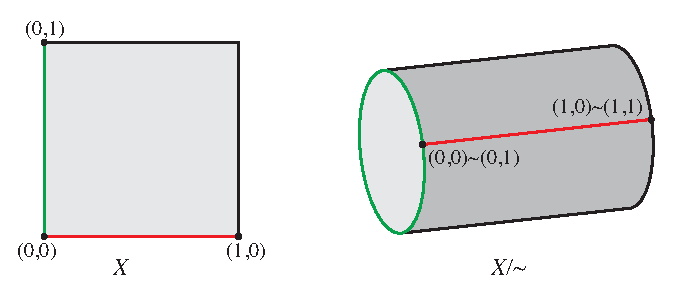
\includegraphics[width=320pt]{images/quotient_spaces/square_to_cylinder}\]
\end{example}
\begin{example}
	Let $X = \R^{2}$ and suppose $(x,y)\sim(x',y')$ if and only if $\exists n,m \in \Z$ such that $x = x' + n, y = y' + m$. 
\end{example}

Note that $X$ may be divided into integer side length squares, such that under $\sim$ all of the given squares are equivalent. Thus we need only consider one such square, noting that the opposite sides are equivalent, yielding a torus. This is pretty much the same as the above example, except that we roll up the cylinder too. In the picture, we are identifying all lines of the same color.
\[
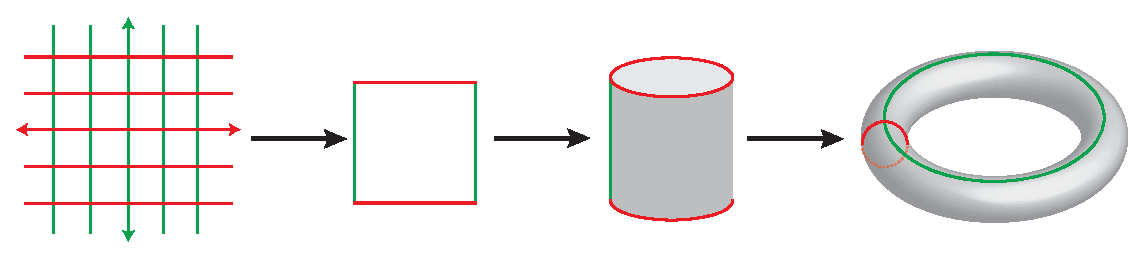
\includegraphics[width=400pt]{images/quotient_spaces/r2_torus}\]

We may also generalize this idea to higher dimensions, yielding the analogous torus for that dimension (i.e. $X = \R^{3}$ yields a 3-torus and so on). 
\begin{example}
	Let $S^{n} = \{x \in \R^{n+1}\ |\ \|x\| = 1\}.$ Define $x \sim y \Leftrightarrow x = \pm y$. 
\end{example}

Note that for $n=1$ we obtain the unit circle such that points connected by a diameter are equivalent. Thus any semi-circle forms a fundamental domain. Such a semicircle has it's endpoints as equivalent, and is thus topologically equivalent to the original circle.

We denote the quotient space $S^{n}/\sim$ by $\RP^{n}$, or the real projective space. The above argument concludes that $\RP^{1} \cong S^{1}$. 
\begin{example}
	From the above, $\RP^{2} = S^{2}/\sim$. We simply note that the fundamental domain is a hemisphere whose boundary takes on the same topology as $\RP^1$ since it is a circle under $\sim$. 
\end{example}
\begin{example}
	Let $X=\R^{2}$ and define $(x,y)\sim(x',y') \Leftrightarrow x^{2}+y^{2}=x^{'2}+y^{'2}$.
	
	Under $\sim$, any points on a circle centered at the origin are equivalent. Collapsing all such circles to points, we find that $X/\sim$ is a ray emanating from the origin (it's pink in the picture).
	\[
	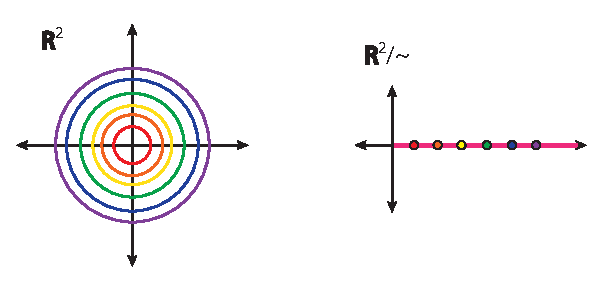
\includegraphics[width=360pt]{images/quotient_spaces/r2_ray}\]
\end{example}
\begin{definition}
	Let $X,Y$ be sets and $f: X \to Y$ be a function. We define the relation $\sim$ {\bf induced by $f$} as follows:
	
	\[\forall p,q \in X, p \sim q \Leftrightarrow f(p)=f(q)\]
	
	It is clear that $\sim$ is an equivalence relation on X because $=$ is an equivalence relation on Y. 
\end{definition}
\begin{definition}
	Suppose $(X,F_{X})$ is a topological space and Y is a set. Let $f: X \to Y$ be onto. Then the {\bf quotient topology} on Y with respect to f is given by: 
	\begin{center}
		$F_{f}=\{U \subseteq Y | f^{-1}(U) \in F_{X}\}$ 
	\end{center}
	If Y has this topology we say that f is a {\bf quotient map}. 
\end{definition}
\begin{tinyfact}
	\begin{enumerate}
		\item $(Y,F_f)$ is a topological space. 
		\item $f: (X,F_X) \rightarrow (Y,F_f)$ is continuous. 
	\end{enumerate}
\end{tinyfact}
\proof Left as an exercise. 
\begin{example}
	Let $f$ map the closed segment $[0,1]$ to a figure-eight, where $f(0)=f(1)=f(\frac{1}{2})$ at the intersection of the two sides of the figure-eight. What is open in the quotient topology $(Y,F_f)$? 
\end{example}
\begin{itemize}
	\item Any open-looking interval on the eight that does not contain the intersection point is open since its preimage is clearly open on the segment; for the same reason, any appropriate union or intersection of these open intervals is also open. 
	\item Furthermore, any open set in the figure-eight that includes the point at the cross must also contain an open interval of nonzero length extending along each of the four legs of the figure-eight. This is necessary because the definition of $F_f$ requires that the preimage of anything open must be open itself; hence the only way for the preimage of a set containing the intersection point to be open is if the preimage is an open set in $[0,1]$ containing the three preimages of the intersection point ($0$, $\frac{1}{2}$, and $1$). 
\end{itemize}

\[
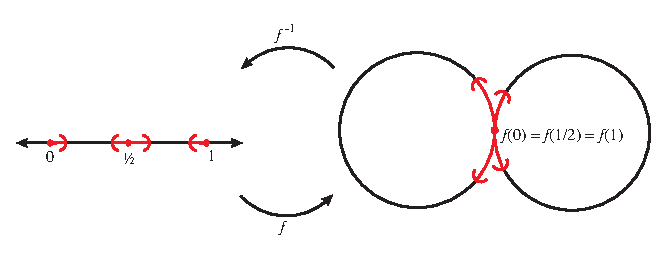
\includegraphics[width=360pt]{images/quotient_spaces/figure_eight_open_sets}\]
\begin{theorem}
	Let $(X,F_X)$ be a topological space, $f: X \twoheadrightarrow Y$ onto, and $\sim$ induced by $f$. Then $(Y,F_f) \cong (X/\sim,F_\sim)$. 
\end{theorem}

If a diagram commutes, then the path taken does not affect the result. Note that the arrow representing $g$ is dashed because we have not yet shown that the diagram commutes. In the proof, we will define $g$ so that the diagram does commute.

\[ \xymatrix{ X \ar[rr]^f \ar[ddr]^\pi & & Y \\
\\
& X/\sim \ar@{-->}[uur]^g } \]
\begin{proof}
	Define $g \colon X/\sim \rightarrow Y$ by $g([\pi]) = f(x)$ where $x$ is a representative of equivalence class $[\pi]$. We want to show that $f$ is well-defined, one-to-one, onto, continuous, and open. 
	\begin{itemize}
		\item Well-defined: WTS if $[x]=[y]$, then $g([x])=g([y])$. That is, any representative of a given equivalence class maps to the same value. Suppose $[x]=[y]$. Then $x \sim y$; since $\sim$ is the relation induced by $f$, $f(x)=f(y)$. $\therefore$ $g([x])=g([y])$. 
		\item One-to-one: Suppose $g([x])=g([y])$. Then $f(x)=f(y)$ $\Rightarrow$ $x \sim y$ $\Rightarrow$ $[x]=[y]$. 
		\item Onto: Suppose $y \in Y$. $f$ is onto, so $\exists x \in X$ such that $f(x)=y$. So $g([x]) = f(x) = y$. 
		\item Continuous: WTS $U \in F_f$ $\Rightarrow$ $g^{-1}(U) \in F_\sim$. Suppose $U \in F_f$. Recalling that $F_\sim = \{ O \subseteq X/\sim \text{ st. } \pi^{-1}(O) \in F_X \}$, we equivalently WTS that $\pi^{-1}(g^{-1}(U)) \in F_X$. Since $U \in F_f$ $\Leftrightarrow$ $f^{-1}(U) \in F_X$, we WTS $f^{-1}(U) = \pi^{-1}(g^{-1}(U))$. 
		\begin{itemize}
			\item[$(\subseteq)$] Let $x \in f^{-1}(U)$. Hence $f(x) = g([x]) \in U$. Since $\pi^{-1}(g^{-1}(U)) = \{ p \text{ st. } g \circ \pi (p) \in U \}$, $g \circ \pi (x) = g([x]) \in U$ $\Rightarrow$ $x \in \pi^{-1}(g^{-1}(U))$. 
			\item[$(\supseteq)$] Let $x \in \pi^{-1}(g^{-1}(U))$. Hence $g(\pi(x)) \in U$ $\Rightarrow$ $g([x]) \in U$ $\Rightarrow$ $f(x) \in U$. So $x \in f^{-1}(U)$. 
		\end{itemize}
		$\therefore$ $f^{-1}(U) = \pi^{-1}(g^{-1}(U))$. Since $f^{-1}(U) \in F_X$, $\pi^{-1}(g^{-1}(U)) \in F_X$. Thus $g^{-1}(U) \in F_\sim$. 
		\item Open: WTS $U \in F_\sim$ $\Rightarrow$ $g(U) \in F_f$. Suppose $U \in F_\sim$. Recalling that $F_f = \{ O \subseteq Y \text{ st. } f^{-1}(O) \in F_X \}$ and that $U \in F_\sim$ $\Leftrightarrow$ $\pi^{-1}(U) \in F_X$, we equivalently WTS $f^{-1}(g(U)) = \pi^{-1}(U)$. 
		\begin{itemize}
			\item[$(\subseteq)$] Let $x \in f^{-1}(g(U))$. So $f(x)=g([x]) \in g(U)$. Since $g$ is bijective (from the earlier parts of this proof), $[x] \in U$ $\Rightarrow$ $\pi(x) \in U$ $\Rightarrow$ $x \in \pi^{-1}(U)$. 
			\item[$(\supseteq)$] Let $x \in \pi^{-1}(U)$. So $\pi(x) \in U$, implying that $g(\pi(x)) \in g(U)$. Then $g(\pi(x)) = g([x]) = f(x)$ $\Rightarrow$ $x \in f^{-1}(g(U))$. 
		\end{itemize}
	\end{itemize}
	Therefore $g$ is a homeomorphism, and $(Y,F_f) \cong (X/\sim,F_\sim)$. 
\end{proof}
\begin{theorem}
	Let $(X,F_X)$ be a topological space and $\sim$ an equivalence relation. Let $Y = X/\sim$ and let $f : X \rightarrow Y$ be $\pi$. Then $F_\sim = F_f$ and $f$ is a quotient map. 
\end{theorem}
\begin{proof}
	Recall that: 
	\begin{align*}
		F_\sim &= \{ U \subseteq X/\sim \text{ st. } \pi^{-1} (U) \in F_x \} \\
		F_f &= \{ U \subseteq Y \text{ st. } f^{-1} (U) \in F_x \}. 
	\end{align*}
	We know that $X/\sim = Y$ and $f = \pi$. $\therefore$ $F_\sim = F_f$. Also, $f = \pi$ is onto since it is a projection, and by definition $F_\sim = F_f$ is a quotient topology. $\therefore$ $f$ is a quotient map. 
\end{proof}
\begin{lemma}
	(Important Lemma about Quotients)\\
	Let $(X,F_X)$, $(Z,F_Z)$ be topological spaces and let $Y$ be a set. Suppose $f: X \twoheadrightarrow Y$ is onto and let $g: (Y,F_f) \rightarrow (Z,F_Z)$. Then $g$ is continuous if and only if $g \circ f$ is continuous. 
\end{lemma}
\begin{proof}
	\begin{itemize}
		\item[$(\Rightarrow)$]: Suppose that $g$ is continuous. Since $f$ is a quotient map, it is continuous. Therefore, $g\circ f$ is a composition of continuous functions, and so $g\circ f$ is continuous.
		
		\item[$(\Leftarrow)$]: Suppose, now, that $g\circ f$ is continuous. Let $U\in F_Z$. Then $(g\circ f)^{-1}(U)\in F_X$. Therefore, $(g\circ f)^{-1}(U) = f^{-1}(g^{-1}(U)) \in F_X$.
		
		Recall that $F_f = \{ V\subseteq Y : f^{-1}(V)\in F_X\}$. So, $g^{-1}(U) \in F_f$, and $g$ is continuous. 
		\begin{flushright}
			$\blacksquare$ 
		\end{flushright}
	\end{itemize}
\end{proof}
\begin{example}
	(A Non-Example)\\
	Let $f: \mathbb{R}-\{1\} \rightarrow \mathbb{R}$ by
	\[ f(x) = 
	\begin{cases}
		x^2 & x\in(-\infty, 1) \\
		\frac{-1}{x-1} & x\in (1, \infty) 
	\end{cases}
	\]
	$f$ is continuous. Let $g: \mathbb{R} \rightarrow \mathbb{R}$ by
	\[ g(x) = 
	\begin{cases}
		1 & x\ge 0 \\
		-1 & x < 0 
	\end{cases}
	\]
	$g$ is not continuous. But $g \circ f: \mathbb{R}-\{1\} \rightarrow \mathbb{R}$ is defined by
	\[ (g\circ f)(x) = 
	\begin{cases}
		-1 & x > 1 \\
		1 & x < 1 
	\end{cases}
	\]
	$g \circ f$ is continuous. 
\end{example}
Question: Does this contradict the Important Lemma?

Answer: No! The solution is, of course, that $g$ actually \emph{is} continuous - the topology of its domain isn't the usual topology. Instead, it has the topology induced by $f$. That is,
\[F_f = \{ U\subseteq \R : f^{-1}(U)\text{ open in }\R\setminus\{1\} \}\]
More precisely, we have $g^{-1}(\{ 1\}) = [0, \infty)$ and $f^{-1}([0, \infty)) = (-\infty,1)$, which is open.

Also, $g^{-1}( \{-1 \} ) = (-\infty,0)$ and $f^{-1}((-\infty, 0)) = (1, \infty)$, which again is open.

Therefore, $g$ is continuous (as we only need to look at the range of $g$, which is $\{-1, 1\}$). 
\begin{theorem}
	Let $(A, F_A)$ and $(B, F_B)$ be topological spaces and $f:A\to B$ be a homeomorphism. Let $\sim_A$ and $\sim_B$ be equivalence relations on $A$ and $B$, respectively, such that $x\sim_A x'$ if and only if $f(x) \sim_B f(x')$.
	
	Then $A/\sim_A \equiv B/\sim_B$. 
\end{theorem}
\begin{proof}
	We want to show that there is some function $g$ such that the following diagram commutes:
	\[ \xymatrix{ A \ar[rr]^f \ar[dd]_{\pi_A} && B \ar[dd]^{\pi_B} \\
	&&\\C \ar @{-->}[rr]_g & & D } \]
	
	\item Define $g:A/\sim_A \to B/\sim_B$ by $g\left([x]_A\right) = \left[ f(x) \right]_B$. To show it's a homeomorphism: 
	\begin{itemize}
		\item {\bf Well-defined:} Suppose $[y]_A = [z]_A$. Then
		\[y\sim_A z\qquad\Rightarrow\qquad f(y) \sim_B f(z) \qquad\Rightarrow \qquad[f(y)]_B = [f(z)]_B]\]
		and so $g$ is well-defined. 
		\item {\bf 1-to-1:} Suppose that $[x]_A$ and $[y]_A$ are such that $g([x]_A) = g([y]_A)$. Then
		\[ [f(x)]_B = [f(y)]_B\quad\Rightarrow\quad f(x)\sim_B f(y)\quad\Rightarrow\quad x\sim_A y \quad\Rightarrow\quad [x]_A = [y]_A\]
		and so $g$ is 1-to-1. 
		\item {\bf Onto: } Let $[y]_B\in B/\sim_B$, and let $x = f^{-1}(y)$. Then
		\[ g([x]_A) = [f(x)]_B = [y]_B \]
		and $g$ is onto. 
		\item {\bf Continuous: } We want to show that $g\circ \pi_A$ is continuous, so we can use the Important Lemma. By the definition of $g$, $g\circ \pi_A = \pi_B\circ f$. Since $f$ is a homeomorphism, it is continuous; $\pi_B$ is a quotient map and is thus continuous. So $\pi_B\circ f$ is continuous. Since $g\circ \pi_A = \pi_B\circ f$, we know that $g\circ \pi_A$ is continuous. As $\pi_A$ is a quotient map, it is continuous, so from the Important Lemma, $g$ is continuous. 
		\item {\bf Open: } We can show equivalently that $g^{-1}$ is continuous instead, since $g$ is a bijection. 
		\begin{align*}
			g\circ\pi_A &= \pi_B\circ f \\
			g^{-1}\circ(g\circ\pi_A)\circ f^{-1} &= g^{-1}\circ(\pi_B\circ f)\circ f^{-1} \\
			\pi_A\circ f^{-1} & =g^{-1}\circ \pi_B 
		\end{align*}
		From here, the argument is eerily similar to the argument for continuity above.
		
		Note that $\pi_A$ is a quotient map and $f^{-1}$ s a homeomorphism, so both are continuous. As such, $\pi_A\circ f^{-1}$ is continuous, and therefore so is $g^{-1}\circ \pi_B$. Since $\pi_B$ is a quotient map, it is continuous; from the Important Lemma, $g^{-1}$ is continuous. Therefore, $g$ is open. 
	\end{itemize}
	Therefore, $g$ is a homeomorphism. Hurrah! 
\end{proof}
